% ==============================================================================
% PERANCANGAN SISTEM (BAB 3 METODOLOGI PENELITIAN)
% Subbab: 3.2 atau 3.X Perancangan Sistem
% Penulis: Rendy Lexxy Kurniawan (NRP 5024231007)
% Terintegrasi dengan:
% - Gambar di: assets/diagrams/
% - Sitasi di: docs/references.bib
% ==============================================================================

\subsection{Perancangan Sistem}
\label{subsec:perancangan_sistem}

Perancangan sistem pada penelitian ini bertujuan untuk mengintegrasikan antarmuka kios interaktif, gateway komunikasi, pengelola siklus hidup (\textit{orchestrator}), serta modul alokasi sumber daya (\textit{resource management}) ke dalam arsitektur berbasis \textit{microservices} yang beroperasi secara lokal pada satu unit perangkat \textit{edge} \cite{chen2022minideep, hossain2023role}. Kios cerdas ini dirancang untuk mengeksekusi beragam layanan kecerdasan buatan heterogen---meliputi pemrosesan percakapan interaktif, analisis citra rekomendasi busana, simulasi video busana langsung (\textit{virtual try-on}), dan pembuatan foto (\textit{AI photobooth})---dengan batasan komputasi fisik satu kartu grafis NVIDIA RTX 5060 berkapasitas 8~GB VRAM \cite{woo2025exploring}. Untuk memberikan pemahaman struktural yang komprehensif, perancangan sistem didekomposisi menjadi empat sub-arsitektur: arsitektur umum sistem secara menyeluruh, arsitektur antarmuka pengguna berbasis peramban Chromium, arsitektur orkestrator layanan, serta arsitektur pengelolaan sumber daya komputasi GPU.

% ------------------------------------------------------------------------------
% 3.X.1 Arsitektur Umum
% ------------------------------------------------------------------------------
\subsubsection{Arsitektur Umum}
\label{subsubsec:arsitektur_umum}

Arsitektur umum sistem smart kiosk dirancang mengikuti pola arsitektur modular terdistribusi lokal (\textit{edge microservices}), di mana setiap komponen memiliki batas tanggung jawab fungsional yang terisolasi dan berkomunikasi melalui kontrak antarmuka pemrograman aplikasi standar \cite{velepucha2023survey}. Sistem ini menghubungkan aliran interaksi manusia-mesin dari lapisan fisik terluar hingga ke lapisan eksekusi kernel kartu grafis lokal, sebagaimana diilustrasikan pada Gambar~\ref{fig:arsitektur_umum}.

\begin{figure}[htbp]
    \centering
    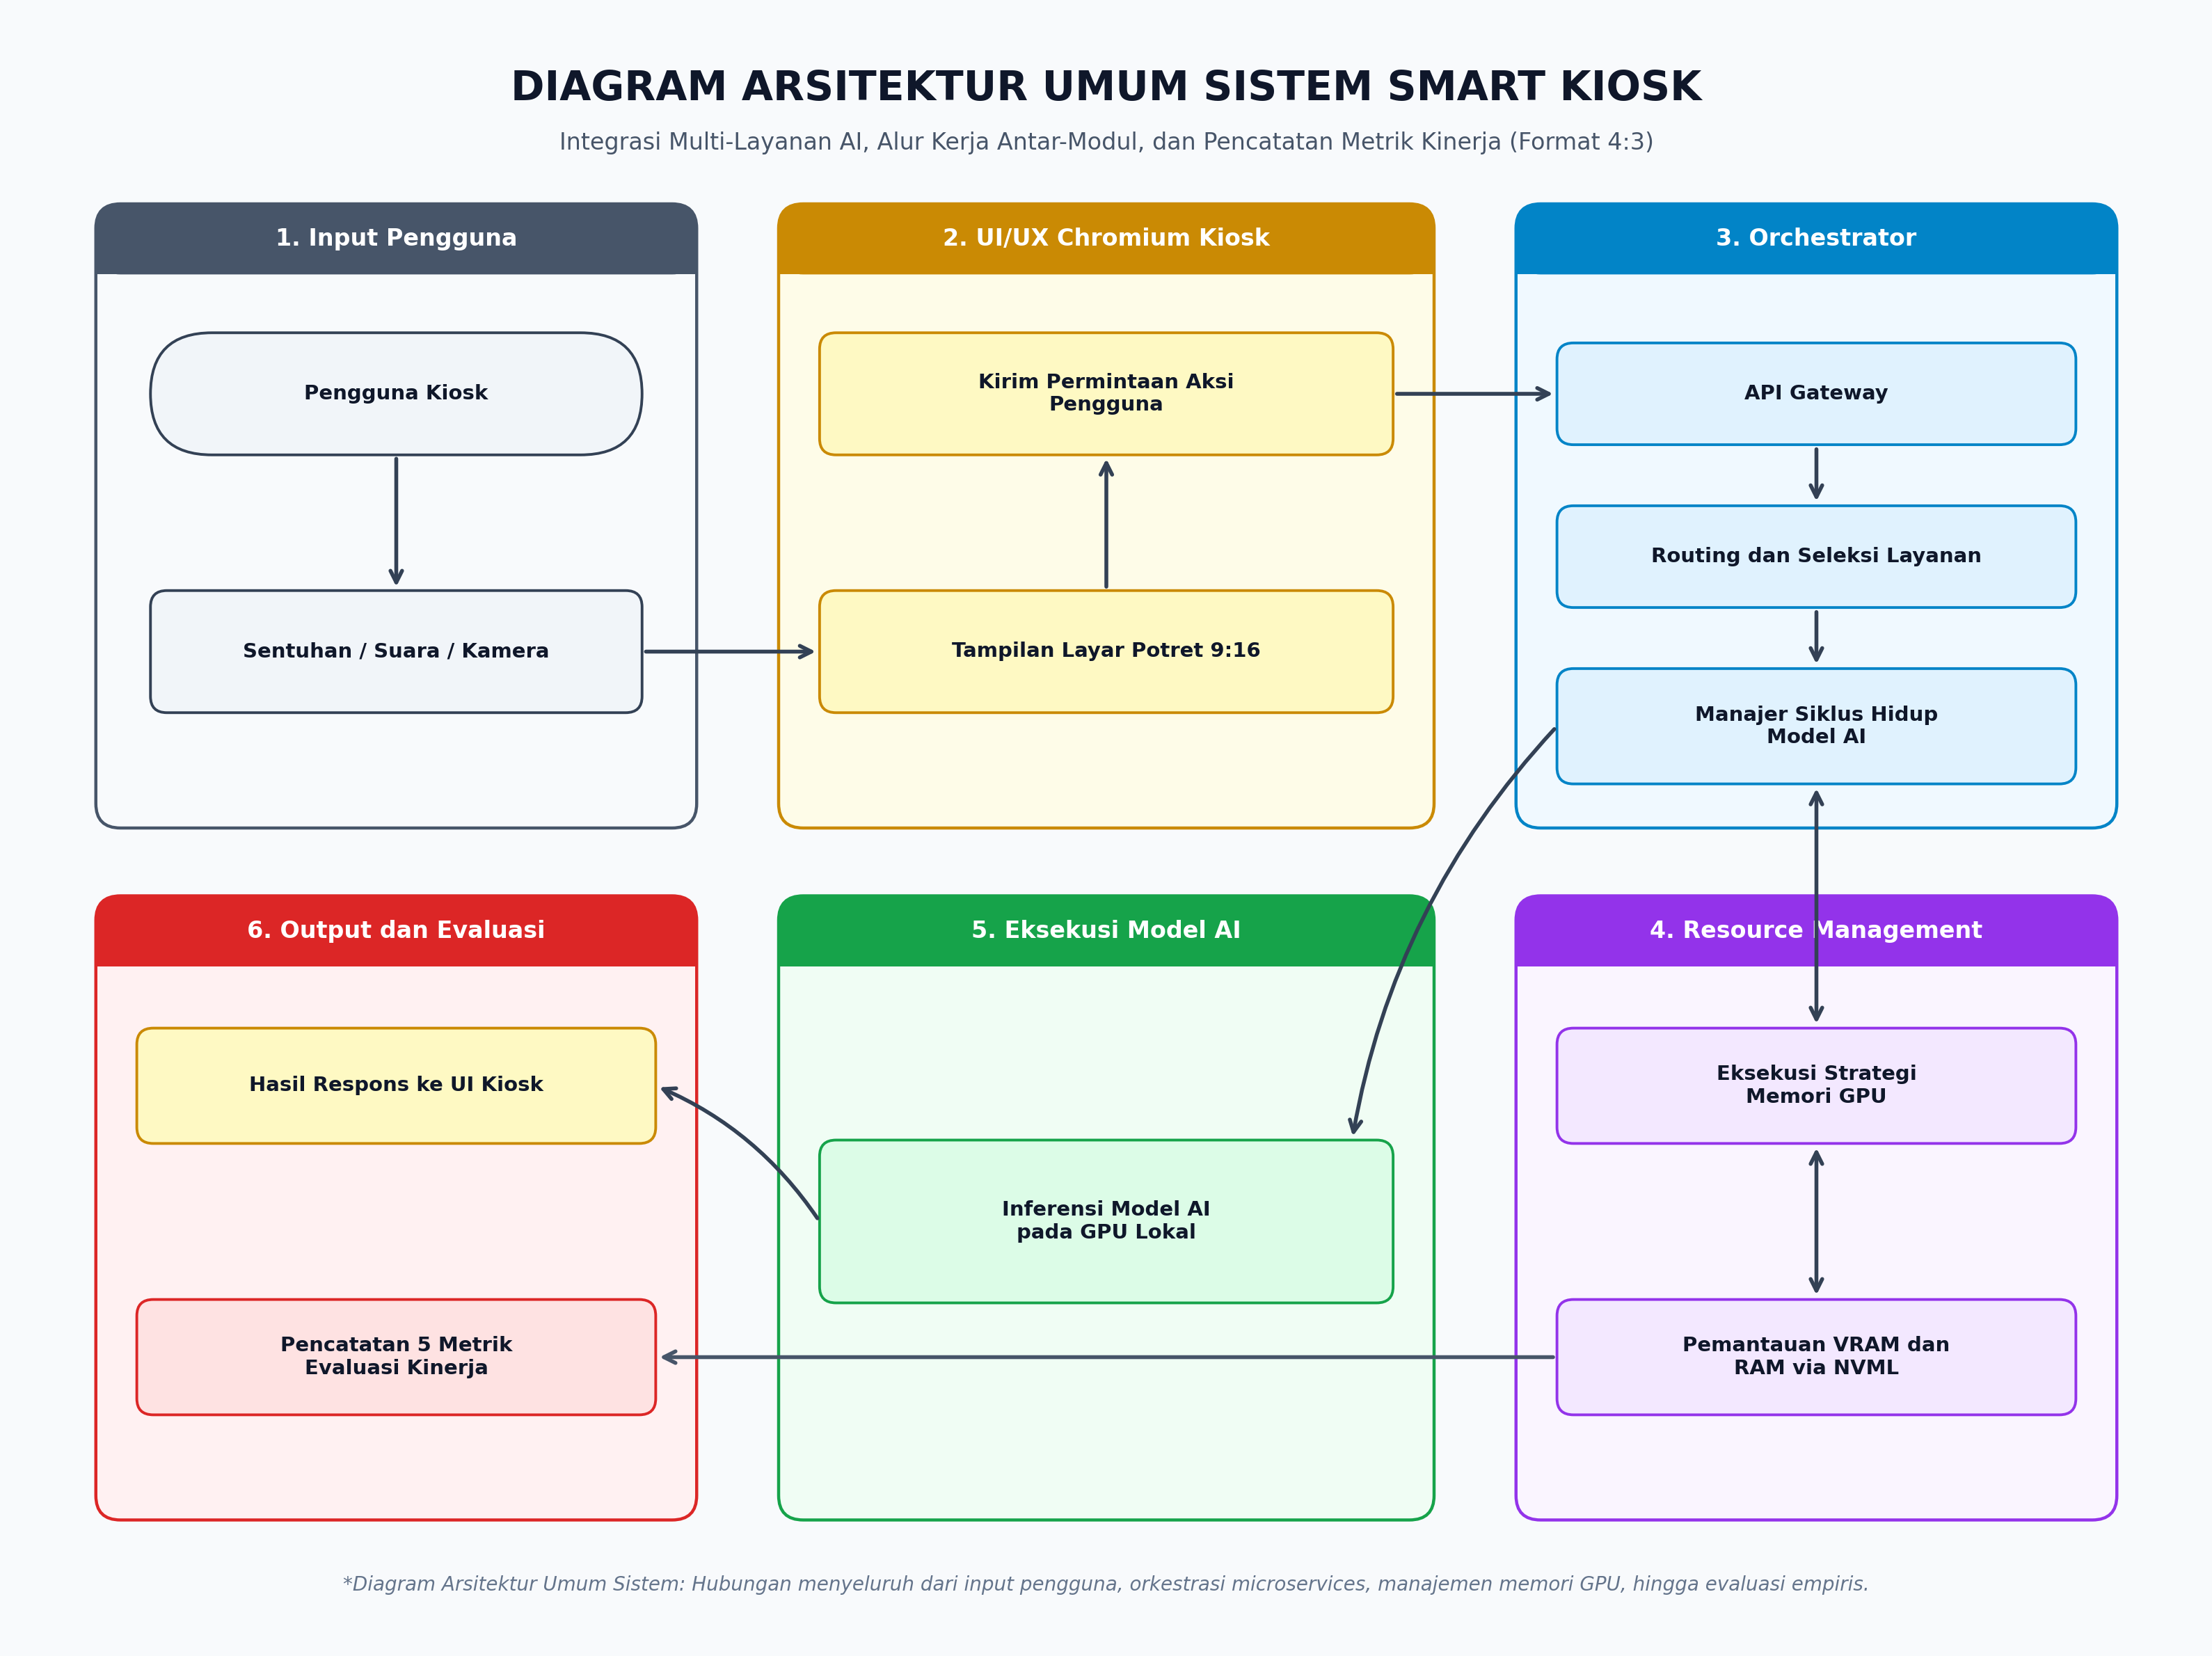
\includegraphics[width=\textwidth]{assets/diagrams/bab3_01_arsitektur_umum.png}
    \caption{Diagram Arsitektur Umum Sistem Orkestrasi Smart Kiosk.}
    \label{fig:arsitektur_umum}
\end{figure}

Aliran pemrosesan sistem terbagi ke dalam enam tahapan utama yang terhubung secara sekuensial dan asinkronus. Tahap pertama dimulai dari penangkapan masukan fisik pengguna melalui sensor sentuhan layar, sinyal audio mikrofon, atau umpan video kamera USB \cite{chen2022minideep}. Masukan tersebut diterima oleh aplikasi antarmuka Chromium kios (Tugas Besar 1) yang menyajikan tampilan berorientasi potret 9:16 dan meneruskan permintaan aksi pengguna ke lapisan gerbang perantara (\textit{API Gateway}). Pada lapisan inti, orkestrator (Tugas Besar 2) bertindak sebagai pengendali sentral yang melakukan validasi permintaan, perutean dinamis (\textit{routing}), dan pengaturan mesin status siklus hidup model (\textit{lifecycle state machine}) \cite{chiang2023management}.

Untuk mencegah kegagalan akibat keterbatasan memori fisik, orkestrator bekerja sama secara erat dengan modul \textit{resource management} (Tugas Besar 3). Modul ini bertanggung jawab mengeksekusi strategi pemindahan bobot memori (Strategi A, B, C, atau D) serta secara simultan memantau kapasitas memori VRAM dan RAM menggunakan pustaka \textit{NVIDIA Management Library} (NVML) \cite{nvidia2026containertoolkit}. Setelah model target diverifikasi berada dalam kondisi siap (\texttt{READY}), eksekusi inferensi matematis dijalankan pada GPU lokal RTX 5060. Keluaran pemrosesan selanjutnya dikembalikan ke antarmuka pengguna untuk ditampilkan secara interaktif, sementara data operasional direkam secara otomatis ke dalam berkas log evaluasi kinerja berdasarkan lima metrik inti \cite{zhang2025adaptive}.

% ------------------------------------------------------------------------------
% 3.X.2 Arsitektur UI/UX Aplikasi Chromium
% ------------------------------------------------------------------------------
\subsubsection{Arsitektur UI/UX Aplikasi Chromium}
\label{subsubsec:arsitektur_ui_ux}

Antarmuka pengguna smart kiosk dirancang khusus untuk layar sentuh vertikal 32 inci beresolusi Full HD ($1080 \times 1920$ piksel) dengan mengadopsi teknologi aplikasi web modern yang dijalankan melalui peramban Chromium dalam mode kios layar penuh (\textit{fullscreen kiosk mode}) \cite{chromium2026kiosk}. Pendekatan peramban terisolasi ini dipilih guna menjamin kestabilan penyajian antarmuka grafis, mempermudah adaptasi tata letak responsif, serta mendukung penerimaan aliran data multimedia (seperti WebRTC dan WebSocket) tanpa menimbulkan konflik pada subsistem grafis Linux host \cite{fette2011websocket}. Alur pengalaman pengguna (\textit{user experience flow}) dari saat mendekati kios hingga memperoleh keluaran layanan AI disajikan pada Gambar~\ref{fig:alur_pengguna_ui}.

\begin{figure}[htbp]
    \centering
    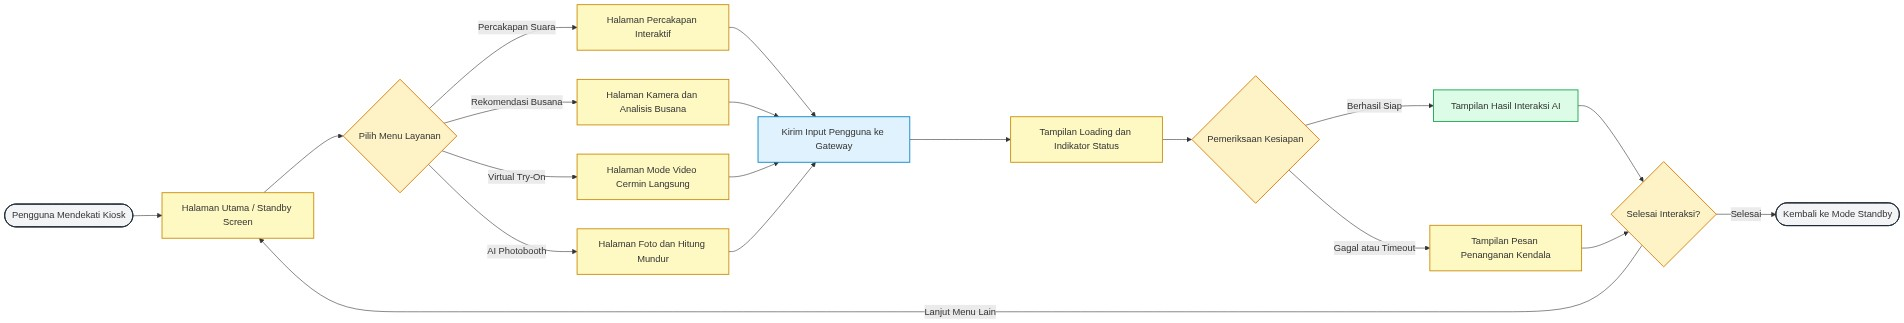
\includegraphics[width=\textwidth]{assets/diagrams/bab3_02_alur_pengguna_ui.png}
    \caption{Diagram Alur Pengalaman Pengguna (\textit{User Flow}) pada UI/UX Kios Chromium.}
    \label{fig:alur_pengguna_ui}
\end{figure}

Perjalanan pengguna diawali dari layar siaga (\textit{standby screen}) yang menampilkan visual animasi interaktif untuk menarik atensi calon pengguna yang berada di zona deteksi kios. Saat pengguna berinteraksi dengan layar sentuh, antarmuka menyajikan menu utama yang memuat empat opsi domain layanan: Percakapan Suara Interaktif, Rekomendasi Busana, \textit{Virtual Try-On}, atau \textit{AI Photobooth} \cite{chen2022minideep}. Setiap menu mengarahkan pengguna ke halaman interaksi spesifik yang dirancang secara ergonomis, memungkinkan pengguna memberikan masukan ucapan suara, berpose di depan kamera pandang potret, atau memilih parameter busana secara intuitif.

Ketika pengguna mengirimkan aksi masukan, antarmuka secara otomatis beralih ke status pemuatan (\textit{loading state}) yang menampilkan indikator progres visual dan status tahapan transisi model secara transparan \cite{chiang2023management}. Melalui koneksi WebSocket asinkronus, antarmuka menerima pembaruan berkala dari gerbang backend mengenai kesiapan layanan target \cite{fette2011websocket}. Jika model AI telah berhasil dimuat dan diverifikasi siap, antarmuka merender hasil keluaran secara langsung---berupa sintesis audio percakapan, galeri citra rekomendasi busana, atau cermin video interaktif \textit{try-on}. Apabila terjadi anomali pemrosesan atau batas waktu terlampaui (\textit{timeout}), antarmuka menampilkan pesan mitigasi kendala yang memandu pengguna untuk mencoba kembali tanpa memicu malafungsi pada aplikasi secara keseluruhan, sebelum akhirnya kembali ke mode siaga saat sesi selesai.

% ------------------------------------------------------------------------------
% 3.X.3 Arsitektur Orchestrator
% ------------------------------------------------------------------------------
\subsubsection{Arsitektur Orchestrator}
\label{subsubsec:arsitektur_orchestrator}

Orkestrator bertindak sebagai pengendali logika dan koordinator operasional utama yang menjembatani lapisan antarmuka pengguna dengan proses-proses model AI lokal \cite{chiang2023management}. Dikembangkan menggunakan bahasa pemrograman Python dan kerangka kerja FastAPI \cite{fastapi2026}, orkestrator mengimplementasikan mesin status siklus hidup (\textit{lifecycle state machine}) terpadu yang mengatur transisi lima status diskrit model: \texttt{STOPPED}, \texttt{STARTING}, \texttt{READY}, \texttt{STOPPING}, dan \texttt{ERROR}. Mekanisme ini memastikan bahwa pemanggilan fungsi inferensi hanya dapat dilakukan apabila alokasi bobot model telah terpasang sempurna di dalam memori komputasi \cite{min2023sensix}. Alur kerja operasional orkestrator diilustrasikan pada Gambar~\ref{fig:alur_kerja_orchestrator}.

\begin{figure}[htbp]
    \centering
    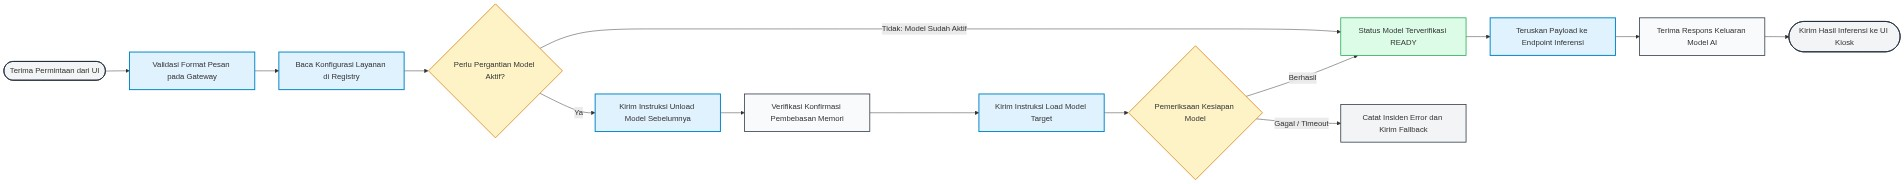
\includegraphics[width=\textwidth]{assets/diagrams/bab3_03_alur_kerja_orchestrator.png}
    \caption{Diagram Alur Kerja Operasional \textit{AI Service Orchestrator}.}
    \label{fig:alur_kerja_orchestrator}
\end{figure}

Alur pemrosesan orkestrator dimulai ketika permintaan aksi pengguna diterima oleh \textit{API Gateway} via endpoint RESTful atau kanal WebSocket \cite{fastapi2026}. Orkestrator memvalidasi integritas muatan data masukan (\textit{payload}) dan mencocokkan konfigurasi layanan yang diminta dengan basis data registri layanan (\texttt{services.yaml}). Registri ini memuat metadata penting mencakup pengenal model, estimasi konsumsi VRAM dasar, metode eksekusi, serta hak eksklusivitas penggunaan kartu grafis \cite{velepucha2023survey}. Selanjutnya, orkestrator memeriksa status model target di dalam VRAM; jika model yang diminta sudah aktif, orkestrator langsung mengalirkan muatan data ke endpoint inferensi tanpa menimbulkan jeda waktu pemuatan tambahan \cite{zhang2025adaptive}.

Sebaliknya, apabila layanan target memerlukan pergantian model atau peralihan ke mode visual eksklusif, orkestrator mengaktifkan protokol pertukaran terkontrol (\textit{controlled swap protocol}) \cite{woo2025exploring}. Orkestrator terlebih dahulu mengirimkan instruksi pelepasan (\textit{unload}) pada model lama, menunggu konfirmasi pembebasan memori, lalu menerbitkan perintah pemuatan (\textit{load}) bagi model target. Untuk memastikan keandalan sistem, orkestrator menjalankan pemeriksaan kesiapan (\textit{readiness check}) berkala pada endpoint \texttt{GET /health} hingga layanan mengembalikan respons kode \texttt{HTTP 200 (Ready)}. Jika inisialisasi berhasil, status layanan diperbarui menjadi \texttt{READY} dan masukan data diteruskan ke mesin inferensi; jika terjadi kegagalan alokasi atau batas waktu terlampaui, orkestrator secara otomatis mencatat insiden kegagalan ke dalam log sistem dan mengeksekusi prosedur pemulihan aman (\textit{graceful fallback}) guna mencegah kegagalan sistemik pada kios cerdas \cite{hossain2023role}.

% ------------------------------------------------------------------------------
% 3.X.4 Arsitektur Resource Management
% ------------------------------------------------------------------------------
\subsubsection{Arsitektur Resource Management}
\label{subsubsec:arsitektur_resource_management}

Arsitektur manajemen sumber daya (\textit{resource management}) dirancang untuk mengendalikan, mengoptimasi, dan memantau pemanfaatan perangkat keras fisik komputasi lokal---terutama memori video GPU (VRAM), memori utama sistem (Host RAM), dan jalur transfer PCIe---secara adaptif dalam batasan kapasitas kartu grafis 8~GB VRAM \cite{woo2025exploring, zhang2025adaptive}. Modul ini bekerja di bawah kendali orkestrator untuk mengeksekusi strategi alokasi memori yang ditentukan sekaligus menjalankan instrumentasi pengukuran kinerja sistem secara terprogram tanpa membebani siklus komputasi inferensi utama \cite{hu2023cec}. Alur kerja operasional modul manajemen sumber daya disajikan pada Gambar~\ref{fig:alur_kerja_resource_management}.

\begin{figure}[htbp]
    \centering
    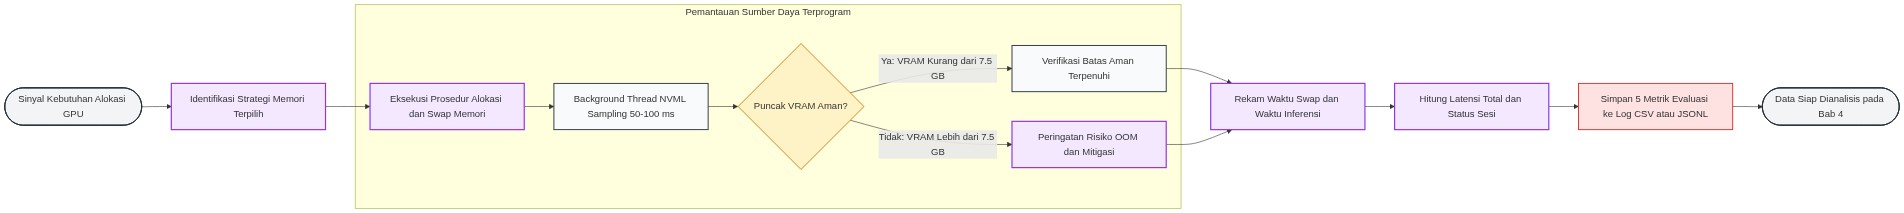
\includegraphics[width=\textwidth]{assets/diagrams/bab3_04_alur_kerja_resource_management.png}
    \caption{Diagram Alur Kerja Operasional Modul \textit{Resource Management} dan Evaluasi.}
    \label{fig:alur_kerja_resource_management}
\end{figure}

Alur kerja dimulai saat modul menerima sinyal kebutuhan alokasi memori dari orkestrator ketika terjadi perpindahan giliran pemrosesan atau pergantian mode interaksi kios. Modul mengidentifikasi strategi memori yang sedang dievaluasi (Strategi A \textit{All-Resident}, Strategi B \textit{Naive Load/Unload}, Strategi C \textit{Pinned-Memory Swap}, atau Strategi D \textit{Prefetch}) dan mengeksekusi prosedur pemindahan data bobot model yang bersesuaian melalui media penyimpanan SSD, Host Pinned RAM, maupun transfer langsung via bus PCIe 4.0 x8 DMA \cite{hu2023cec, woo2025exploring}. Bersamaan dengan proses tersebut, utas latar belakang (\textit{background monitoring thread}) yang memanfaatkan pustaka \textit{NVIDIA Management Library} (NVML) diaktifkan untuk mencuplik pemakaian memori fisik GPU secara kontinu setiap interval 50--100~ms \cite{nvidia2026containertoolkit}.

Siklus pemantauan ini secara aktif melakukan verifikasi ambang batas keselamatan untuk memastikan alokasi VRAM puncak tidak melampaui batas kritis yang ditetapkan ($V_{\text{peak}} \le 7{,}5\text{ GB}$). Mekanisme ini menjamin tersedianya ruang pengaman (\textit{headroom}) minimal sebesar 500~MB guna mencegah terjadinya kegagalan memori meluap (\textit{CUDA Out of Memory}) yang dapat menghentikan sistem secara fatal \cite{min2023sensix}. Selama siklus interaksi berjalan, modul mencatat waktu transisi pertukaran model ($T_{\text{swap}}$) dan waktu inferensi murni ($T_{\text{infer}}$), mengagregasikan total latensi interaksi ujung-ke-ujung ($T_{\text{e2e}}$), serta memeriksa status keberhasilan sesi guna menghitung tingkat kestabilan operasional (\textit{Stability Rate} / $SR$) \cite{zhang2025adaptive}. Seluruh hasil pengukuran lima metrik kinerja ini disimpan secara terstruktur ke dalam berkas log benchmark (format CSV dan JSONL) sebagai basis data empiris yang siap dianalisis dan dibahas pada Bab IV \cite{chen2022minideep}.
